\section{Ejercicio 4 (otro de Programacion dinamica):}

En este ejercicio nos piden resolver el problema usando otro algoritmo de programacion dinamica. En nuestro caso lo vamos a realizar en base al anterior ejercicio pero vamos a hacerlo recursivo.

Habiamos visto que teniamos que buscar cual era la mejor combinacion de ultimo rojo y ultimo azul, para el anterior ejercicio estabamos calculando la matriz constructivamente, lo haciamos de una forma que cuando necesitabamos un subproblema ya sabiamos que lo teniamos solucionado. Ahora lo que vamos a hacer es, no nos importa el orden en el que lo calculamos, pero cuando lo pido y no lo tengo, recursivamente me pongo a calcularlo, obviamente la matriz la mantenemos, asi no calculamos algo 2 veces. Entonces lo unico que tenemos que hacer es preguntar cuando vale cada el emento de la matriz en cualquier orden y si los subproblemas necesarios no estan calculados se calculan recursivamente.

\begin{algorithm}[H]
\NoCaptionOfAlgo
	\KwData{	
	arreglo = el arreglo de numeros entero\\
	n = el tamaño del arreglo\\
	\KwResult{La cantidad minima de numeros sin pintar para una secuencia de numeros de largo n}
	\caption{\algoritmo{ej3}{int arreglo[], n}{int}}
		\tcc{Creamos nuestra matriz y esta toda inicializada en -1}
		int m[n+1][n+1]\\

		\tcc{Le guardamos los triviales, los del primer indice(0)}
		int m[0][n] $\leftarrow$ n - 1\\
		int m[n][0] $\leftarrow$ n - 1\\
		int m[n][n] $\leftarrow$ n \\

		int optimo $\leftarrow$ n\\

		\tcc{Recorremos todos los indices buscando el optimo}
		\For(){$i \leftarrow 0$ \KwTo n}{
			\For(){$j \leftarrow 0$ \KwTo n}{
				\If{(i != j || i == n) \textbf{and} optimo(i,j) < optimo}{
					optimo $\leftarrow$ optimo(i,j) 
				}
			}
		}

		res $\leftarrow$ optimo
	}
\end{algorithm}

\begin{algorithm}[H]
\NoCaptionOfAlgo
	\KwData{	
	Suponemos que tiene acceso al arreglo a la matriz y al largo\\
	r = El indice que estamos pintando de rojo\\
	a = El indice que fijamos de azul\\
	\KwResult{El optimo para m[r][a]}
	\caption{\algoritmo{optimo}{int r, a}{int}}
		\tcc{Nos fijamos si esta calculado}
		\If{m[r][a] = -1}{
			\tcc{Si no esta calculado hay que calcularlo}
			\tcc{Ahora nos tenemos revisamos cual fijar}

			\eIf{(ultimoAzul $<$ ultimoRojo  \textbf{and} ultimoRojo != largo)  \textbf{or} ultimoAzul = largo}{
		        m[ultimoRojo][ultimoAzul] $\leftarrow$ buscarOptimoRojo(ultimoRojo, ultimoAzul);
			}{
		        m[ultimoRojo][ultimoAzul] $\leftarrow$  buscarOptimoAzul(ultimoAzul, ultimoRojo);
			}

		
		}
		\tcc{Devolvemos el numero calculado}
		res $\leftarrow$ m[r][a]
	}
\end{algorithm}

\begin{algorithm}[H]
\NoCaptionOfAlgo
	\caption{\algoritmo{buscarOptimoPintandoDeRojo}{int r, a}{int}}
		\tcc{Como defecto ponemos el largo del arreglo}
		int optimoActual $\leftarrow$ largo\\
		\tcc{Recorremos con el azul fijado, que pasaria si partieramos desde los anteriores rojos}
		\For(){$ri \leftarrow 0$ \KwTo r - 1}{
			\tcc{Nos fijamos si el numero de la secuencia de ri es menor al de r,(osea si podemos pintarlo a partir de ri), y si es mas chico que el optimoActual}
			\If{ri != a \textbf{and} arreglo[ri] $<$ arreglo[r] \textbf{and} m[ri][a] $<$ optimoActual}{
				\tcc{Si es menor, marcamos a este como el optimoActual}
				optimoActual $\leftarrow$ m[ri][a]
			}
		}
		\tcc{Retornamos el optimo del cual podemos pintar y como pintamos este ultimo se reduce en 1}
		res $\leftarrow$ optimoActual - 1 
	
\end{algorithm}


\subsection*{Analisis de Complejidad}
Basicamente es la misma que en la de del ejercicio 3. Recorremos todos los numeros de la matriz y solos lo vamos a calcular una vez, y en el peor de los casos calcular este numero es $O(n)$. Podemos notar que dependiendo de que se pregunta primero, vamos a tener algunos datos primeros que otro. Por ejemplo si empezamos por los ultimos indices se va a calcular toda la matriz. Y despues cuando recorramos toda vamos a tener todos los datos en$O(1)$

\subsection*{Experimentación Computacional}
\subsubsection*{Instancias Aleatorias}
De vuelta usamos las mismas instancias que antes, generadas para el ejercicio 1.

\begin{center}
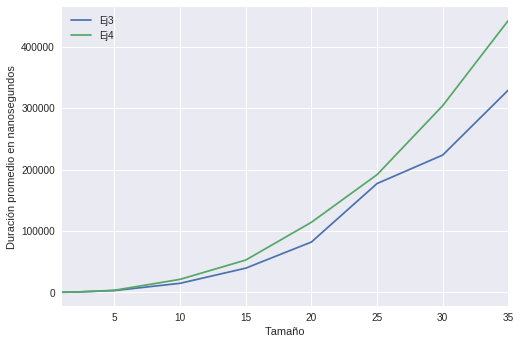
\includegraphics[scale=0.5]{ej4Random1-40.png}\\
\end{center}

Podemos notar que son muy similares(hacen casi los mismos calculos), pero podemos notar que este nueva implementacion, esto se puede deber a que ya que es recursiva gastamos memoria teniendo las llamadas, o a algun tema con la implementacion que lo empeoro.
